%%%%%
%% Compile using LuaLaTeX
%% Use Biber as Bibliography Tool
%% This document is in version: `DRAFT'.
%%%%%

\documentclass{cgu}

%%%%% General Comments
%%% Citations
%% For adding your references, add a `references.bib'
%% Include url only if doi is not provided
%% For textual citation use \citet{id} = author (year)
%% For parental citation use \citep{id} = (author year)
%%% Images
%% For adding your images, put the files as img/filename.extension
%%%%%

\hypersetup{
	pdfauthor={},
	pdftitle={},
	pdfcreator={}
}

\title{Title}
\author{Full Name\thanks{
		Affiliation: Institution\\Corresponding Author: \href{mailto:local-part@domain.name}{local-part@domain.name}
	}
}

\begin{document}

\maketitle

\begin{abstract}
This is a textual citation \citet{Einstein1905}. This is the same, but parental \citep{Einstein1905}.
\end{abstract}

%%%
%% Line spacing to 1.5
\onehalfspacing
%%%

\begin{table}[!hbpt]
    \caption{Table Captions Above Table}
    \centering
\begin{tabularx}{0.5\textwidth}{Y Y}
    a   &   c\\
    b   &   d
\end{tabularx}
\\
\raggedright
\footnotesize
\emph{\\Source:} Here I tell you where I got this.\\
\emph{Explanation:} This is where I talk about it briefly.

    \label{tab:Table1}
\end{table}

\begin{figure}[!hbpt]
    {\centering
    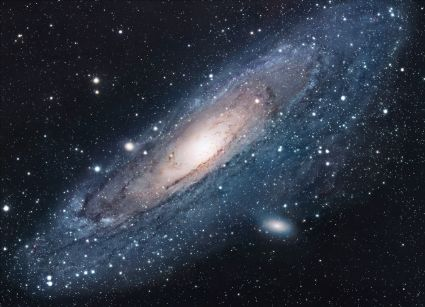
\includegraphics{universe}
    }\\
    \raggedright
    \footnotesize
    \emph{\\Source:} Here I tell you where I got this.\\
    \emph{Explanation:} This is where I talk about it briefly.
    \caption{Figures Caption Below Figure}
    \label{fig:Figure1}
\end{figure}

%%%
\singlespacing
%%%

\printbibliography

\end{document}